\documentclass[windows,csize4]{BHCexam}
%\documentclass[windows,csize4,answers]{BHCexam}

\usepackage{multicol} % 分栏
\usepackage{polynom} % 多项式除法
\pagestyle{fancy}
\fancyfoot[C]{\kaishu \small 第 \thepage 页 共 \pageref{lastpage} 页}
%\fancyhead[L]{\includegraphics[width=2cm]{qrcode.png}}
\title{光的直线传播和反射}
%\subtitle{数学文科试卷}
%\notice{满分150分, 120分钟完成, \\	允许使用计算器,答案一律写在答题纸上.}
%\author{Gavin Chen}
%\date{\today}
\usepackage{enumerate} % 编号
\usepackage{cases}
\usepackage{subfigure}
\usepackage{graphicx}

\begin{document}

\maketitle

\begin{groups}
    \group{光的直线传播}{}
    \begin{itemize}
        \item 光在同种均匀介质中沿直线传播。(为什么?费马原理,最小作用量原理,变分法。)
        \item 直线传播的例子:影子,月食,日食,小孔成像。
        \item 光源的概念:能发出一定波长范围的电磁波(包括可见光以及紫外线、红外线和X射线等不可见光)的物体。
        \item 冷光源和热光源:一般来说,冷光源发光不会对周围温度产生明显变化。通常利用化学能,生物能来转化为光能。而热光源通常发光同时也会发热。
        \item 自然光源,人造光源。
    \end{itemize}

    补充知识: 费马原理(Fermat's principle)光传播的路径是光程取极值的路径。这个极值可能是极大值、极小值,甚至是函数的拐点。
    费马原理更正确的称谓应是“平稳时间原理”:光沿着所需时间为平稳的路径传播。所谓的平稳是数学上的微分概念,可以理解为一阶导数为零,它可以是极大值、极小值甚至是拐点。
    \begin{itemize}
        \item 平面镜:任意两点的反射路径光程是最小值。
        \item 半椭圆形镜子:其两个焦点的光线反射路径不是唯一的,光程都一样,是最大值,也是最小值。
        \item 半圆形镜子:其两个端点Q、P的反射路径光程是最大值。
    \end{itemize}

    光源发光照到不透明物体后,在物体背光面形成的光所达不到的区域即为影子。
    影区是发自光源并于被照物体相切的光线围成的。图\ref{fig:fig_3_1}(a)中,点光源形成的影。如果把点光源改成面光源,如图\ref{fig:fig_3_1}(b)所示。
    注意这时候情况会有所不同,后面的影区氛围本影(完全照不到)和半影(部分照到)。
    想一想,假如图\ref{fig:fig_3_1}(b)中光源为圆形,的半影区有个人往光源看,他看到的光源是什么形状?
    \begin{figure}[htb]
        \centering
        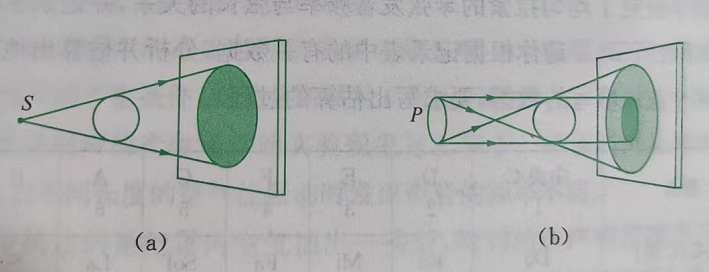
\includegraphics [scale=0.75,trim=0 0 0 0]{./image/fig_3_1.PNG}
        \caption{点光源与面光源的影}
        \label{fig:fig_3_1}
    \end{figure}

    图\ref{fig:fig_3_2}所示为日食情况。a为本影区,看到日全食;c、d为半影区,看到日偏食;而b为伪本影区,看到日环食。
    \begin{figure}[htb]
        \centering
        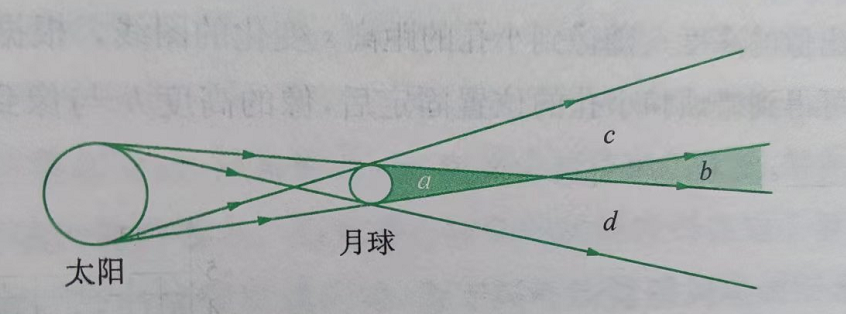
\includegraphics [scale=0.5,trim=0 0 0 0]{./image/fig_3_2.PNG}
        \caption{日食}
        \label{fig:fig_3_2}
    \end{figure}
    图\ref{fig:fig_3_3}所示为月食情况。想一想,为什么没有月环食?
    \begin{figure}[htb]
        \centering
        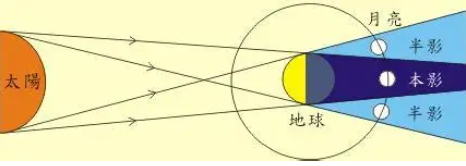
\includegraphics [scale=0.75,trim=0 0 0 0]{./image/fig_3_3.PNG}
        \caption{月食}
        \label{fig:fig_3_3}
    \end{figure}

    \group{光的反射}{}
    \begin{itemize}
        \item 光从一种介质射向另一种介质表面时,有部分光返回原介质的传播现象称之为光的反射。
        \item 光射到水面,玻璃等许多物体表面时,都有反射现象。
    \end{itemize}

    如图\ref{fig:fig_3_8}所示,激光打在界面上后反射。
    \begin{figure}[htb]
        \centering
        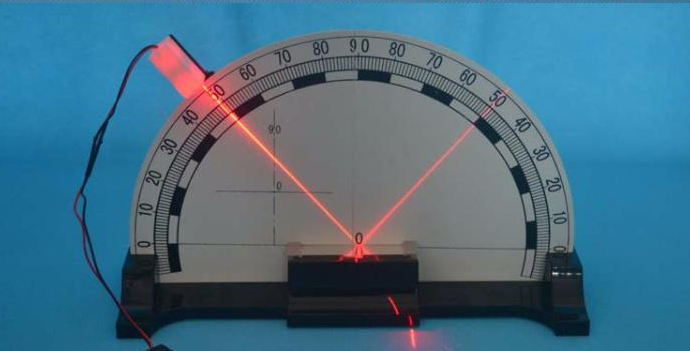
\includegraphics [scale=0.5,trim=0 0 0 0]{./image/fig_3_8.PNG}
        \caption{光的反射}
        \label{fig:fig_3_8}
    \end{figure}

    根据费马原理,平面镜反射的入射角和反射角相等。(将军饮马问题)

    光的反射定律\ref{fig:fig_3_9}:入射光,反射光与法线在同一平面内;反射光线和入射光线分别位于发现的两侧;反射角等于入射角。
    \begin{figure}[htb]
        \centering
        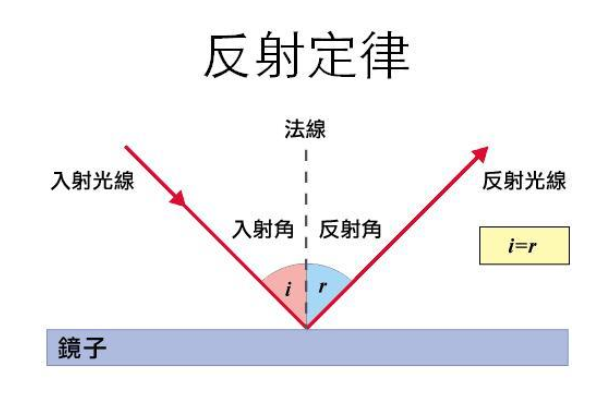
\includegraphics [scale=0.35,trim=0 0 0 0]{./image/fig_3_9.PNG}
        \caption{反射定律}
        \label{fig:fig_3_9}
    \end{figure}
    注意一定是同一平面内和光路可逆原理。

    镜面反射和漫反射。
    \begin{figure}[htb]
        \centering
        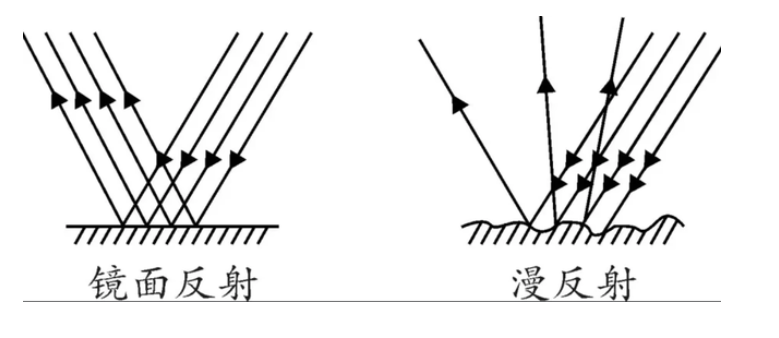
\includegraphics [scale=0.35,trim=0 0 0 0]{./image/fig_3_10.PNG}
        \caption{镜面反射和漫反射}
        \label{fig:fig_3_10}
    \end{figure}
    \begin{itemize}
        \item 镜面反射:平行光入射到物体表面后反射光线平行射出。形成条件:反射面光滑。比如镜子,光滑的黑板。
        \item 漫反射:平行光入射到物体表面后反射光线向各个方向射出。形成条件:反射面粗糙。比如电影屏幕,衣服,马路。
    \end{itemize}
    想一想:我们常说反光,说的是哪一种反射?雨后的夜晚,如果迎着月光行走在乡间小路,为了避免踏入水坑,我们一般会选择走暗处的地面,为什么?

    \group{例题}{}

    \begin{questions}[]
        \question[5]如图\ref{fig:fig_3_4}所示。如果作为光源的蜡烛往左移动,小孔成像在屏上的像会变大还是变小?如果屏往左移动,像是变大还是变小?
        \begin{figure}[htb]
            \centering
            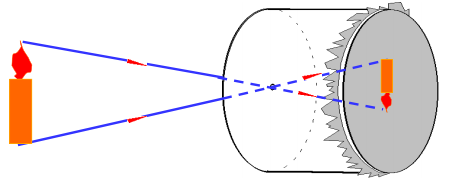
\includegraphics [scale=0.75,trim=0 0 0 0]{./image/fig_3_4.PNG}
            \caption{小孔成像}
            \label{fig:fig_3_4}
        \end{figure}
        \begin{solution}{0.5cm}
            \methodonly 略
        \end{solution}
        \vspace{3cm}

        \question[5] 如图\ref{fig:fig_3_5}所示。路灯距地面的高度$H=8m$,身高$h=1.6m$的人自路灯的正下方经过时,看到自己头部的影子正好在自己脚下。如果人以$v=1m/s$的速度匀速向前走,则人头部的影子的速度是多少?
        \begin{figure}[htb]
            \centering
            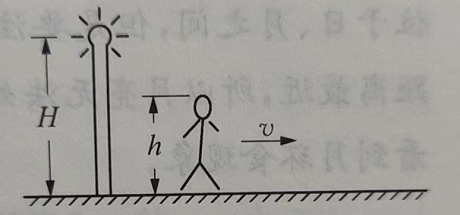
\includegraphics [scale=0.75,trim=0 0 0 0]{./image/fig_3_5.PNG}
            \caption{路灯下行走示意图}
            \label{fig:fig_3_5}
        \end{figure}
        \begin{solution}{0.5cm}
            \methodonly  如图\ref{fig:fig_3_6}。O为路灯位置,从侧面看,假设人从A走到了B的长度,影子从C走了了D位置。$\frac{AB}{CD}=\frac{OA}{OC}=\frac{H-h}{h}$。
            因为$AB=vt$,可以得到$CD=\frac{H}{H-h}\times vt$。而$\frac{H}{H-h}\times v$是不变的,所以影子也是匀速直线运动,即为$\frac{H}{H-h}\times v=1.25m/s$
            \begin{figure}[htb]
                \centering
                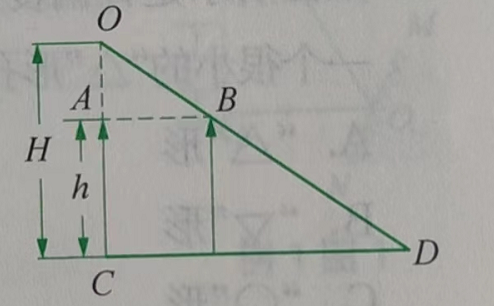
\includegraphics [scale=0.75,trim=0 0 0 0]{./image/fig_3_6.PNG}
                \caption{路灯下行走示意图2}
                \label{fig:fig_3_6}
            \end{figure}
        \end{solution}
        \vspace{3cm}

        \question[5] 小欣和老师一起设计了如图\ref{fig:fig_3_11}的实验装置探究”光的反射定律“。
        \begin{figure}[htb]
            \centering
            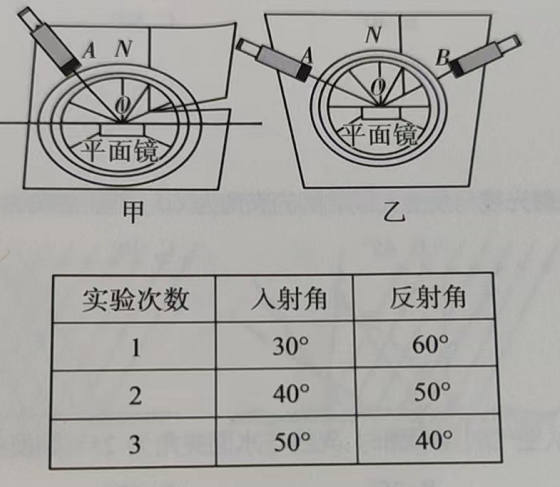
\includegraphics [scale=0.5,trim=0 0 0 0]{./image/fig_3_11.PNG}
            \caption{光的反射定律探究实验}
            \label{fig:fig_3_11}
        \end{figure}
        \begin{subquestions}
            \subquestion 小欣将呈现反射光线的活动卡纸向后折,活动卡片上就看不到反射光线了,这说明什么?
            \subquestion 实验中多次改变入射光线$AO$与$ON$的夹角进行实验,测量记录如表所示。同组小王分析小张记录的入射角正确,但在读反射角数据时有误,你认为可能的原因是什么?
            \subquestion 如图乙所示,再用另一只激光笔让光线沿着 $BO$(即逆着原反射光线)射向平面镜时,可看到反射光线沿$OA$射出,这说明什么?
            \subquestion 在小镜子中看到同桌的眼睛时,你的同桌是否也能看到你的眼睛?请用光学知识解释。
        \end{subquestions}
        \vspace{3cm}

        \question[5] 墙基地面上有一盏发出平行光的灯$S$,墙面前3m的地面上有一个平面镜,如图\ref{fig:fig_3_12}所示。为使地面灯光能照到墙面上离平面镜入射点$O$距离为$6m$的地方,平面镜与地面夹角应是多少?
        \begin{figure}[htb]
            \centering
            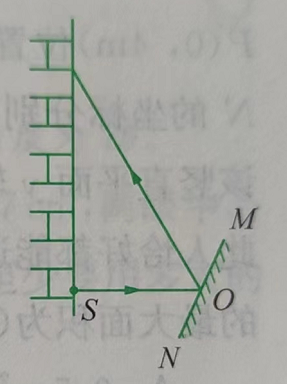
\includegraphics [scale=0.5,trim=0 0 0 0]{./image/fig_3_12.PNG}
            \caption{光与墙面示意图}
            \label{fig:fig_3_12}
        \end{figure}
        \vspace{3cm}

        \question[5]如图\ref{fig:fig_3_13}所示,在竖直平面$xOy$内,人眼位于$P(0,4m)$位置处,平面镜$MN$竖直放置,其两端$M$、$N$的坐标分别为$(3m,1m)$和$(3m,0)$。
        某发光点在该竖直平面y轴的右半部分某一区域内自由移动时,此人恰好都能通过平面镜看见发光点的像,则该区域的最大面积为多少?
        \begin{figure}[htb]
            \centering
            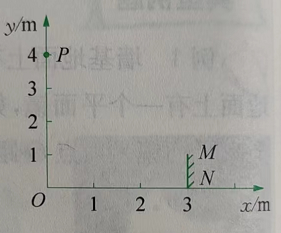
\includegraphics [scale=0.5,trim=0 0 0 0]{./image/fig_3_13.PNG}
            \caption{示意图}
            \label{fig:fig_3_13}
        \end{figure}
        \begin{solution}{0.5cm}
            \methodonly  如图所示,求梯形面积即可,$S=\frac{1}{2}\times (1m+2m)\times 3m=4.5m^2$。
            \begin{figure}[htb]
                \centering
                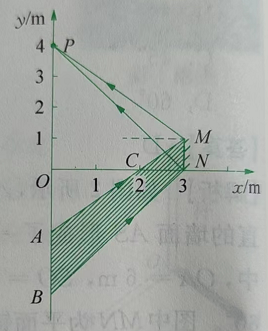
\includegraphics [scale=0.5,trim=0 0 0 0]{./image/fig_3_14.PNG}
                \caption{示意图}
                \label{fig:fig_3_14}
            \end{figure}
        \end{solution}
        \vspace{3cm}
        \question[5] 如图\ref{fig:fig_3_16}所示,两平面镜之间夹角为$35^o$。一束入射光线经两平面镜两次反射,那么入射光线与反射光线的夹角$\theta$是多少?
        \begin{figure}[htb]
            \centering
            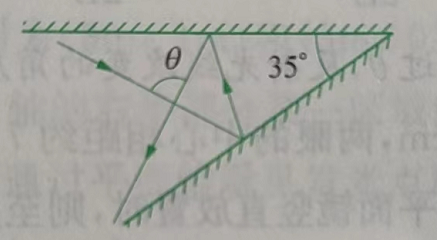
\includegraphics [scale=0.75,trim=0 0 0 0]{./image/fig_3_16.PNG}
            \caption{两平面镜之间的反射}
            \label{fig:fig_3_16}
        \end{figure}
        \begin{solution}{0.5cm}
            \methodonly  略
        \end{solution}
    \end{questions}
\end{groups}


\begin{groups}
    \group{作业}{}
    \begin{questions}[]

        \question[5] 如图\ref{fig:fig_3_7}所示。晴天里,某同学在操场上竖立一根直杆,地面上$OA$是这根杆在太阳光下的投影,过了一段时间后,影子的位置移到了$OB$,$OA=OB$,如图所示。则$AB$所指的方向是什么?
        \begin{figure}[htb]
            \centering
            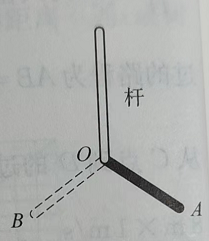
\includegraphics [scale=0.75,trim=0 0 0 0]{./image/fig_3_7.PNG}
            \caption{直杆的影子}
            \label{fig:fig_3_7}
        \end{figure}
        \begin{solution}{0.5cm}
            \methodonly 太阳自东向西,所以影子自西向东。故而$AB$方向向东。想一想,为什么要强调$OA=OB$?
        \end{solution}
        \vspace{3cm}

        \question[5] 一般人脸宽(包括两耳)约$18cm$,两眼的中心相距约$7cm$,两眼中心离头顶和下巴分别为$10cm$和$13cm$。
        当平面镜竖直放置时,则至少要用多大的平面镜(矩形),才能看到自己全部的脸?
        \begin{solution}{0.5cm}
            \methodonly 由于照镜子的时候脸的平面一定平行于镜子,所以镜子边缘一定在眼睛和耳朵连线的中垂线上。显然左眼看右耳并且右眼看左耳才能使镜子最小。
            \begin{figure}[htb]
                \centering
                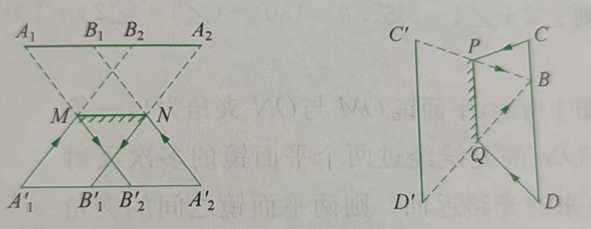
\includegraphics [scale=0.5,trim=0 0 0 0]{./image/fig_3_15.PNG}
                \caption{照镜子示意图}
                \label{fig:fig_3_15}
            \end{figure}
        \end{solution}
        \vspace{3cm}

        \question[5] 如图所示,平面镜$OM$与$ON$夹角为$\theta$,一条平行于平面镜$ON$的光线经过两个平面镜的多次反射后,能够沿着原来的光路返回。
        则两平面镜之间的夹角不可能是\key{$B$}.
        \fourchoices{$20^o$}{$15^o$}{$10^o$}{$5^o$}
        \begin{figure}[htb]
            \centering
            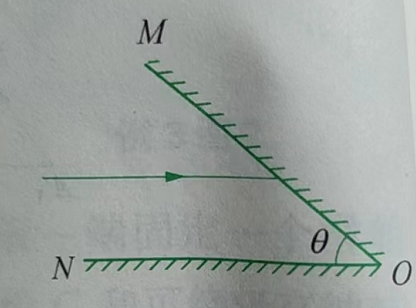
\includegraphics [scale=0.5,trim=0 0 0 0]{./image/fig_3_17.PNG}
            \caption{光线在平面镜见反射}
            \label{fig:fig_3_17}
        \end{figure}
        \begin{solution}{0.5cm}
            \methodonly 略
        \end{solution}


    \end{questions}
\end{groups}
\label{lastpage}
\end{document}